\documentclass[1p]{elsarticle_modified}
%\bibliographystyle{elsarticle-num}

%\usepackage[colorlinks]{hyperref}
%\usepackage{abbrmath_seonhwa} %\Abb, \Ascr, \Acal ,\Abf, \Afrak
\usepackage{amsfonts}
\usepackage{amssymb}
\usepackage{amsmath}
\usepackage{amsthm}
\usepackage{scalefnt}
\usepackage{amsbsy}
\usepackage{kotex}
\usepackage{caption}
\usepackage{subfig}
\usepackage{color}
\usepackage{graphicx}
\usepackage{xcolor} %% white, black, red, green, blue, cyan, magenta, yellow
\usepackage{float}
\usepackage{setspace}
\usepackage{hyperref}

\usepackage{tikz}
\usetikzlibrary{arrows}

\usepackage{multirow}
\usepackage{array} % fixed length table
\usepackage{hhline}

%%%%%%%%%%%%%%%%%%%%%
\makeatletter
\renewcommand*\env@matrix[1][\arraystretch]{%
	\edef\arraystretch{#1}%
	\hskip -\arraycolsep
	\let\@ifnextchar\new@ifnextchar
	\array{*\c@MaxMatrixCols c}}
\makeatother %https://tex.stackexchange.com/questions/14071/how-can-i-increase-the-line-spacing-in-a-matrix
%%%%%%%%%%%%%%%

\usepackage[normalem]{ulem}

\newcommand{\msout}[1]{\ifmmode\text{\sout{\ensuremath{#1}}}\else\sout{#1}\fi}
%SOURCE: \msout is \stkout macro in https://tex.stackexchange.com/questions/20609/strikeout-in-math-mode

\newcommand{\cancel}[1]{
	\ifmmode
	{\color{red}\msout{#1}}
	\else
	{\color{red}\sout{#1}}
	\fi
}

\newcommand{\add}[1]{
	{\color{blue}\uwave{#1}}
}

\newcommand{\replace}[2]{
	\ifmmode
	{\color{red}\msout{#1}}{\color{blue}\uwave{#2}}
	\else
	{\color{red}\sout{#1}}{\color{blue}\uwave{#2}}
	\fi
}

\newcommand{\Sol}{\mathcal{S}} %segment
\newcommand{\D}{D} %diagram
\newcommand{\A}{\mathcal{A}} %arc


%%%%%%%%%%%%%%%%%%%%%%%%%%%%%5 test

\def\sl{\operatorname{\textup{SL}}(2,\Cbb)}
\def\psl{\operatorname{\textup{PSL}}(2,\Cbb)}
\def\quan{\mkern 1mu \triangleright \mkern 1mu}

\theoremstyle{definition}
\newtheorem{thm}{Theorem}[section]
\newtheorem{prop}[thm]{Proposition}
\newtheorem{lem}[thm]{Lemma}
\newtheorem{ques}[thm]{Question}
\newtheorem{cor}[thm]{Corollary}
\newtheorem{defn}[thm]{Definition}
\newtheorem{exam}[thm]{Example}
\newtheorem{rmk}[thm]{Remark}
\newtheorem{alg}[thm]{Algorithm}

\newcommand{\I}{\sqrt{-1}}
\begin{document}

%\begin{frontmatter}
%
%\title{Boundary parabolic representations of knots up to 8 crossings}
%
%%% Group authors per affiliation:
%\author{Yunhi Cho} 
%\address{Department of Mathematics, University of Seoul, Seoul, Korea}
%\ead{yhcho@uos.ac.kr}
%
%
%\author{Seonhwa Kim} %\fnref{s_kim}}
%\address{Center for Geometry and Physics, Institute for Basic Science, Pohang, 37673, Korea}
%\ead{ryeona17@ibs.re.kr}
%
%\author{Hyuk Kim}
%\address{Department of Mathematical Sciences, Seoul National University, Seoul 08826, Korea}
%\ead{hyukkim@snu.ac.kr}
%
%\author{Seokbeom Yoon}
%\address{Department of Mathematical Sciences, Seoul National University, Seoul, 08826,  Korea}
%\ead{sbyoon15@snu.ac.kr}
%
%\begin{abstract}
%We find all boundary parabolic representation of knots up to 8 crossings.
%
%\end{abstract}
%\begin{keyword}
%    \MSC[2010] 57M25 
%\end{keyword}
%
%\end{frontmatter}

%\linenumbers
%\tableofcontents
%
\newcommand\colored[1]{\textcolor{white}{\rule[-0.35ex]{0.8em}{1.4ex}}\kern-0.8em\color{red} #1}%
%\newcommand\colored[1]{\textcolor{white}{ #1}\kern-2.17ex	\textcolor{white}{ #1}\kern-1.81ex	\textcolor{white}{ #1}\kern-2.15ex\color{red}#1	}

{\Large $\underline{12n_{0742}~(K12n_{0742})}$}

\setlength{\tabcolsep}{10pt}
\renewcommand{\arraystretch}{1.6}
\vspace{1cm}\begin{tabular}{m{100pt}>{\centering\arraybackslash}m{274pt}}
\multirow{5}{120pt}{
	\centering
	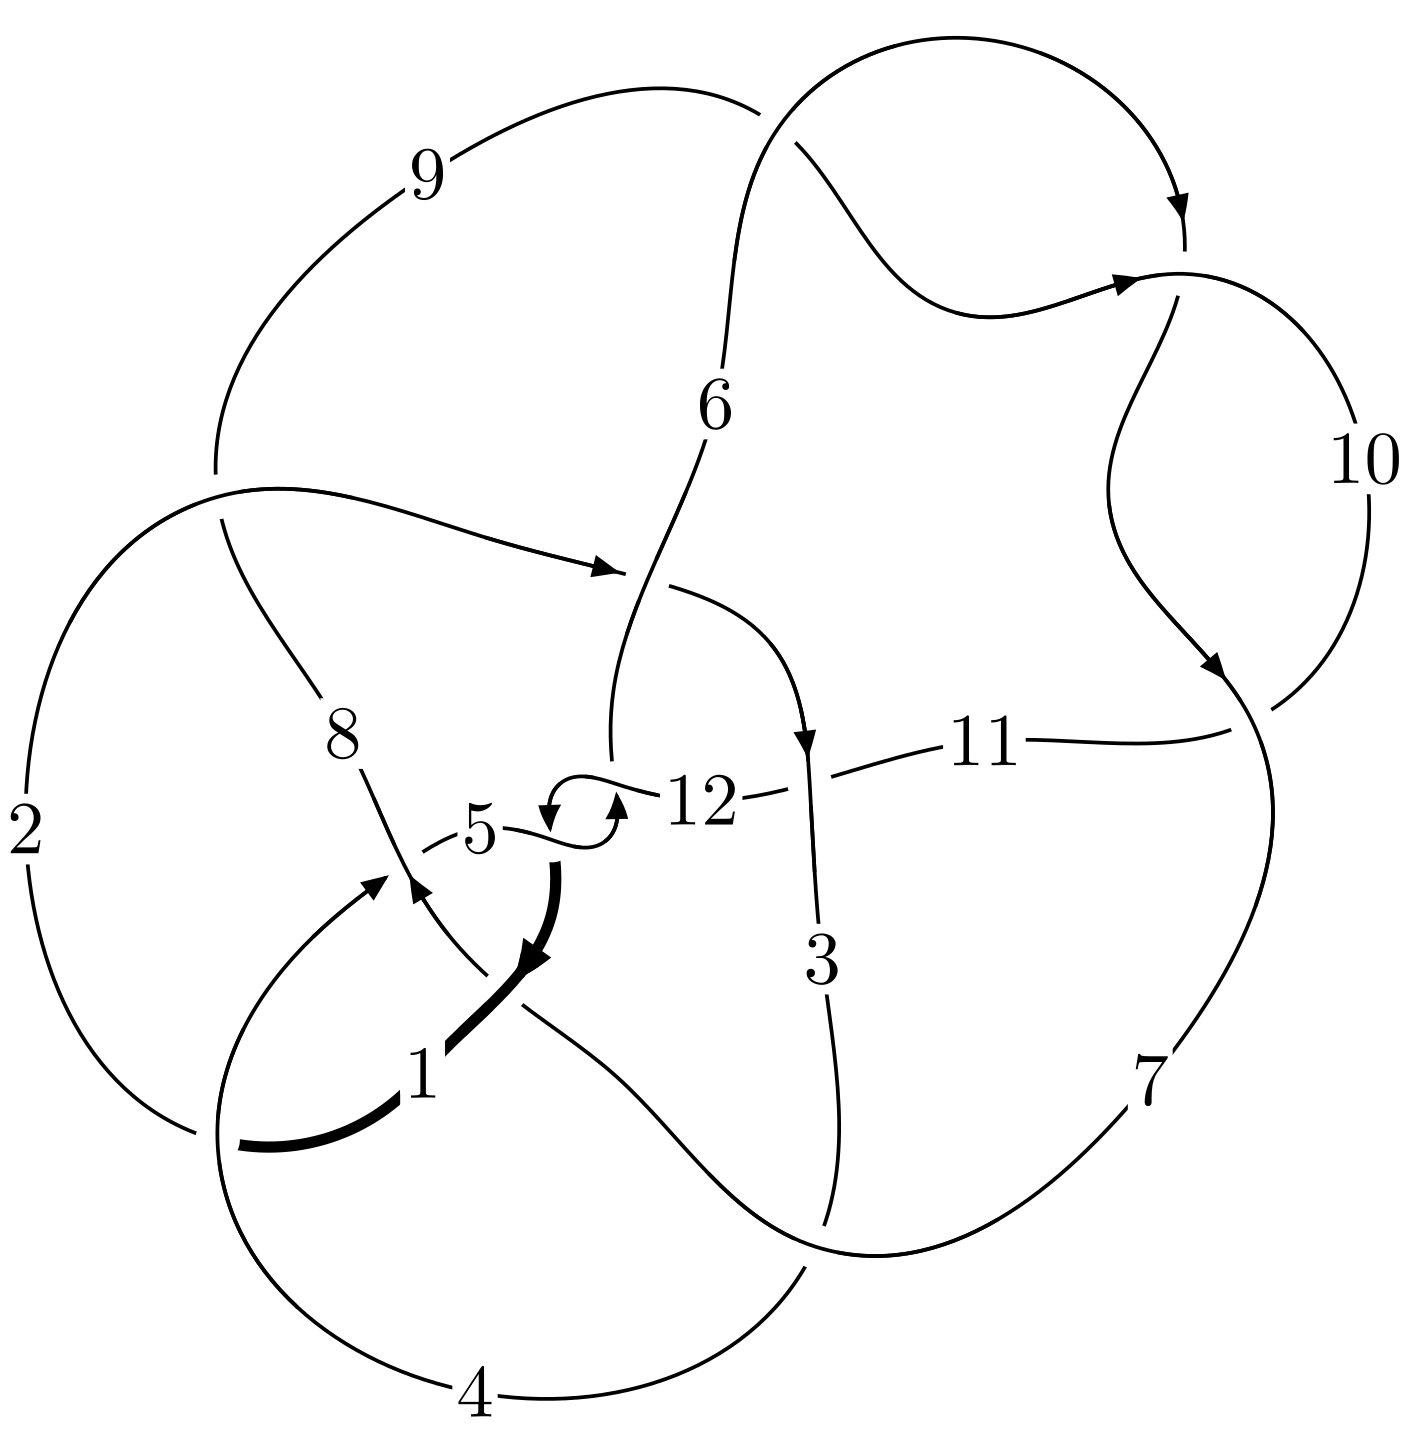
\includegraphics[width=112pt]{../../../GIT/diagram.site/Diagrams/png/2831_12n_0742.png}\\
\ \ \ A knot diagram\footnotemark}&
\allowdisplaybreaks
\textbf{Linearized knot diagam} \\
\cline{2-2}
 &
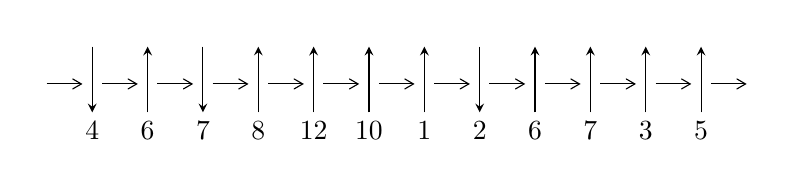
\begin{tikzpicture}[x=20pt, y=17pt]
	% nodes
	\node (C0) at (0, 0) {};
	\node (C1) at (1, 0) {};
	\node (C1U) at (1, +1) {};
	\node (C1D) at (1, -1) {4};

	\node (C2) at (2, 0) {};
	\node (C2U) at (2, +1) {};
	\node (C2D) at (2, -1) {6};

	\node (C3) at (3, 0) {};
	\node (C3U) at (3, +1) {};
	\node (C3D) at (3, -1) {7};

	\node (C4) at (4, 0) {};
	\node (C4U) at (4, +1) {};
	\node (C4D) at (4, -1) {8};

	\node (C5) at (5, 0) {};
	\node (C5U) at (5, +1) {};
	\node (C5D) at (5, -1) {12};

	\node (C6) at (6, 0) {};
	\node (C6U) at (6, +1) {};
	\node (C6D) at (6, -1) {10};

	\node (C7) at (7, 0) {};
	\node (C7U) at (7, +1) {};
	\node (C7D) at (7, -1) {1};

	\node (C8) at (8, 0) {};
	\node (C8U) at (8, +1) {};
	\node (C8D) at (8, -1) {2};

	\node (C9) at (9, 0) {};
	\node (C9U) at (9, +1) {};
	\node (C9D) at (9, -1) {6};

	\node (C10) at (10, 0) {};
	\node (C10U) at (10, +1) {};
	\node (C10D) at (10, -1) {7};

	\node (C11) at (11, 0) {};
	\node (C11U) at (11, +1) {};
	\node (C11D) at (11, -1) {3};

	\node (C12) at (12, 0) {};
	\node (C12U) at (12, +1) {};
	\node (C12D) at (12, -1) {5};
	\node (C13) at (13, 0) {};

	% arrows
	\draw[->,>={angle 60}]
	(C0) edge (C1) (C1) edge (C2) (C2) edge (C3) (C3) edge (C4) (C4) edge (C5) (C5) edge (C6) (C6) edge (C7) (C7) edge (C8) (C8) edge (C9) (C9) edge (C10) (C10) edge (C11) (C11) edge (C12) (C12) edge (C13) ;	\draw[->,>=stealth]
	(C1U) edge (C1D) (C2D) edge (C2U) (C3U) edge (C3D) (C4D) edge (C4U) (C5D) edge (C5U) (C6D) edge (C6U) (C7D) edge (C7U) (C8U) edge (C8D) (C9D) edge (C9U) (C10D) edge (C10U) (C11D) edge (C11U) (C12D) edge (C12U) ;
	\end{tikzpicture} \\
\hhline{~~} \\& 
\textbf{Solving Sequence} \\ \cline{2-2} 
 &
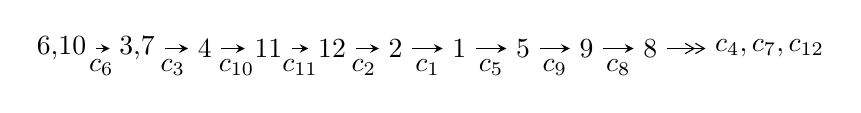
\begin{tikzpicture}[x=23pt, y=7pt]
	% node
	\node (A0) at (-1/8, 0) {6,10};
	\node (A1) at (17/16, 0) {3,7};
	\node (A2) at (17/8, 0) {4};
	\node (A3) at (25/8, 0) {11};
	\node (A4) at (33/8, 0) {12};
	\node (A5) at (41/8, 0) {2};
	\node (A6) at (49/8, 0) {1};
	\node (A7) at (57/8, 0) {5};
	\node (A8) at (65/8, 0) {9};
	\node (A9) at (73/8, 0) {8};
	\node (C1) at (1/2, -1) {$c_{6}$};
	\node (C2) at (13/8, -1) {$c_{3}$};
	\node (C3) at (21/8, -1) {$c_{10}$};
	\node (C4) at (29/8, -1) {$c_{11}$};
	\node (C5) at (37/8, -1) {$c_{2}$};
	\node (C6) at (45/8, -1) {$c_{1}$};
	\node (C7) at (53/8, -1) {$c_{5}$};
	\node (C8) at (61/8, -1) {$c_{9}$};
	\node (C9) at (69/8, -1) {$c_{8}$};
	\node (A10) at (11, 0) {$c_{4},c_{7},c_{12}$};

	% edge
	\draw[->,>=stealth]	
	(A0) edge (A1) (A1) edge (A2) (A2) edge (A3) (A3) edge (A4) (A4) edge (A5) (A5) edge (A6) (A6) edge (A7) (A7) edge (A8) (A8) edge (A9) ;
	\draw[->>,>={angle 60}]	
	(A9) edge (A10);
\end{tikzpicture} \\ 

\end{tabular} \\

\footnotetext{
The image of knot diagram is generated by the software ``\textbf{Draw programme}" developed by Andrew Bartholomew(\url{http://www.layer8.co.uk/maths/draw/index.htm\#Running-draw}), where we modified some parts for our purpose(\url{https://github.com/CATsTAILs/LinksPainter}).
}\phantom \\ \newline 
\centering \textbf{Ideals for irreducible components\footnotemark of $X_{\text{par}}$} 
 
\begin{align*}
I^u_{1}&=\langle 
54417405 u^{24}+534792001 u^{23}+\cdots+33311573 b+3681796776,\\
\phantom{I^u_{1}}&\phantom{= \langle  }32555757366 u^{24}+426906642534 u^{23}+\cdots+2831483705 a+4024705159097,\\
\phantom{I^u_{1}}&\phantom{= \langle  }u^{25}+14 u^{24}+\cdots+802 u+85\rangle \\
I^u_{2}&=\langle 
26555 u^{18}-198357 u^{17}+\cdots+36185 b-144112,\\
\phantom{I^u_{2}}&\phantom{= \langle  }163099 u^{18}-1122706 u^{17}+\cdots+36185 a-527630,\;u^{19}-7 u^{18}+\cdots-7 u+1\rangle \\
I^u_{3}&=\langle 
1445734 u^6 a^5-1807249 u^6 a^4+\cdots-3844804 a+2844990,\;u^6 a^5-2 u^6 a^4+\cdots-37 a+3,\\
\phantom{I^u_{3}}&\phantom{= \langle  }u^7-2 u^6+2 u^5+u^4-2 u^3+3 u^2-2 u+1\rangle \\
I^u_{4}&=\langle 
a^5-5 a^4+5 a^3+5 a^2+7 b-10 a-2,\;a^6- a^5- a^4+4 a^3+3 a^2-1,\;u+1\rangle \\
\\
I^v_{1}&=\langle 
a,\;b^3+b^2-1,\;v-1\rangle \\
\end{align*}
\raggedright * 5 irreducible components of $\dim_{\mathbb{C}}=0$, with total 95 representations.\\
\footnotetext{All coefficients of polynomials are rational numbers. But the coefficients are sometimes approximated in decimal forms when there is not enough margin.}
\newpage
\renewcommand{\arraystretch}{1}
\centering \section*{I. $I^u_{1}= \langle 5.44\times10^{7} u^{24}+5.35\times10^{8} u^{23}+\cdots+3.33\times10^{7} b+3.68\times10^{9},\;3.26\times10^{10} u^{24}+4.27\times10^{11} u^{23}+\cdots+2.83\times10^{9} a+4.02\times10^{12},\;u^{25}+14 u^{24}+\cdots+802 u+85 \rangle$}
\flushleft \textbf{(i) Arc colorings}\\
\begin{tabular}{m{7pt} m{180pt} m{7pt} m{180pt} }
\flushright $a_{6}=$&$\begin{pmatrix}1\\0\end{pmatrix}$ \\
\flushright $a_{10}=$&$\begin{pmatrix}0\\u\end{pmatrix}$ \\
\flushright $a_{3}=$&$\begin{pmatrix}-11.4978 u^{24}-150.771 u^{23}+\cdots-10908.2 u-1421.41\\-1.63359 u^{24}-16.0542 u^{23}+\cdots-598.744 u-110.526\end{pmatrix}$ \\
\flushright $a_{7}=$&$\begin{pmatrix}1\\- u^2\end{pmatrix}$ \\
\flushright $a_{4}=$&$\begin{pmatrix}-1.30031 u^{24}-16.5707 u^{23}+\cdots-3108.43 u-444.101\\-3.38147 u^{24}-53.3166 u^{23}+\cdots-6600.19 u-838.456\end{pmatrix}$ \\
\flushright $a_{11}=$&$\begin{pmatrix}u\\- u^3+u\end{pmatrix}$ \\
\flushright $a_{12}=$&$\begin{pmatrix}6.05270 u^{24}+79.5081 u^{23}+\cdots+5244.89 u+673.380\\2.36945 u^{24}+27.1163 u^{23}+\cdots+502.162 u+69.9568\end{pmatrix}$ \\
\flushright $a_{2}=$&$\begin{pmatrix}-9.86418 u^{24}-134.717 u^{23}+\cdots-10309.5 u-1310.89\\-1.63359 u^{24}-16.0542 u^{23}+\cdots-598.744 u-110.526\end{pmatrix}$ \\
\flushright $a_{1}=$&$\begin{pmatrix}-4.83382 u^{24}-68.1991 u^{23}+\cdots-7333.97 u-961.507\\-3.85589 u^{24}-51.6884 u^{23}+\cdots-3026.16 u-368.196\end{pmatrix}$ \\
\flushright $a_{5}=$&$\begin{pmatrix}-3.32745 u^{24}-47.7352 u^{23}+\cdots-3929.81 u-486.742\\-3.53542 u^{24}-41.2464 u^{23}+\cdots-561.643 u-67.3117\end{pmatrix}$ \\
\flushright $a_{9}=$&$\begin{pmatrix}- u\\u\end{pmatrix}$ \\
\flushright $a_{8}=$&$\begin{pmatrix}4.06599 u^{24}+56.5411 u^{23}+\cdots+7053.62 u+949.032\\5.22968 u^{24}+70.3553 u^{23}+\cdots+4181.88 u+514.479\end{pmatrix}$\\&\end{tabular}
\flushleft \textbf{(ii) Obstruction class $= -1$}\\~\\
\flushleft \textbf{(iii) Cusp Shapes $= \frac{989445234}{33311573} u^{24}+\frac{12906576392}{33311573} u^{23}+\cdots+\frac{940441773198}{33311573} u+\frac{123998150314}{33311573}$}\\~\\
\newpage\renewcommand{\arraystretch}{1}
\flushleft \textbf{(iv) u-Polynomials at the component}\newline \\
\begin{tabular}{m{50pt}|m{274pt}}
Crossings & \hspace{64pt}u-Polynomials at each crossing \\
\hline $$\begin{aligned}c_{1}\end{aligned}$$&$\begin{aligned}
&u^{25}-24 u^{24}+\cdots-1246 u+85
\end{aligned}$\\
\hline $$\begin{aligned}c_{2},c_{11}\end{aligned}$$&$\begin{aligned}
&u^{25}+18 u^{23}+\cdots+10 u+1
\end{aligned}$\\
\hline $$\begin{aligned}c_{3},c_{8}\end{aligned}$$&$\begin{aligned}
&u^{25}-15 u^{23}+\cdots- u-1
\end{aligned}$\\
\hline $$\begin{aligned}c_{4},c_{7}\end{aligned}$$&$\begin{aligned}
&u^{25}- u^{24}+\cdots+u-1
\end{aligned}$\\
\hline $$\begin{aligned}c_{5},c_{12}\end{aligned}$$&$\begin{aligned}
&u^{25}-15 u^{24}+\cdots-768 u+64
\end{aligned}$\\
\hline $$\begin{aligned}c_{6},c_{9},c_{10}\end{aligned}$$&$\begin{aligned}
&u^{25}-14 u^{24}+\cdots+802 u-85
\end{aligned}$\\
\hline
\end{tabular}\\~\\
\newpage\renewcommand{\arraystretch}{1}
\flushleft \textbf{(v) Riley Polynomials at the component}\newline \\
\begin{tabular}{m{50pt}|m{274pt}}
Crossings & \hspace{64pt}Riley Polynomials at each crossing \\
\hline $$\begin{aligned}c_{1}\end{aligned}$$&$\begin{aligned}
&y^{25}-12 y^{24}+\cdots-5534 y-7225
\end{aligned}$\\
\hline $$\begin{aligned}c_{2},c_{11}\end{aligned}$$&$\begin{aligned}
&y^{25}+36 y^{24}+\cdots+36 y-1
\end{aligned}$\\
\hline $$\begin{aligned}c_{3},c_{8}\end{aligned}$$&$\begin{aligned}
&y^{25}-30 y^{24}+\cdots+15 y-1
\end{aligned}$\\
\hline $$\begin{aligned}c_{4},c_{7}\end{aligned}$$&$\begin{aligned}
&y^{25}+9 y^{24}+\cdots+3 y-1
\end{aligned}$\\
\hline $$\begin{aligned}c_{5},c_{12}\end{aligned}$$&$\begin{aligned}
&y^{25}+13 y^{24}+\cdots+30720 y-4096
\end{aligned}$\\
\hline $$\begin{aligned}c_{6},c_{9},c_{10}\end{aligned}$$&$\begin{aligned}
&y^{25}-8 y^{24}+\cdots+28824 y-7225
\end{aligned}$\\
\hline
\end{tabular}\\~\\
\newpage\flushleft \textbf{(vi) Complex Volumes and Cusp Shapes}
$$\begin{array}{c|c|c}  
\text{Solutions to }I^u_{1}& \I (\text{vol} + \sqrt{-1}CS) & \text{Cusp shape}\\
 \hline 
\begin{aligned}
u &= \phantom{-}1.150840 + 0.071771 I \\
a &= -0.388264 + 0.151015 I \\
b &= \phantom{-}0.994844 - 0.281020 I\end{aligned}
 & \phantom{-}3.73403 + 0.45497 I & \phantom{-}9.6713 - 10.3747 I \\ \hline\begin{aligned}
u &= \phantom{-}1.150840 - 0.071771 I \\
a &= -0.388264 - 0.151015 I \\
b &= \phantom{-}0.994844 + 0.281020 I\end{aligned}
 & \phantom{-}3.73403 - 0.45497 I & \phantom{-}9.6713 + 10.3747 I \\ \hline\begin{aligned}
u &= -0.485653 + 0.637254 I \\
a &= \phantom{-}0.238682 - 1.222900 I \\
b &= \phantom{-}0.134188 - 0.806451 I\end{aligned}
 & \phantom{-}0.04540 - 2.20353 I & \phantom{-}6.08023 + 5.72200 I \\ \hline\begin{aligned}
u &= -0.485653 - 0.637254 I \\
a &= \phantom{-}0.238682 + 1.222900 I \\
b &= \phantom{-}0.134188 + 0.806451 I\end{aligned}
 & \phantom{-}0.04540 + 2.20353 I & \phantom{-}6.08023 - 5.72200 I \\ \hline\begin{aligned}
u &= -1.170090 + 0.293084 I \\
a &= -0.088746 + 0.564255 I \\
b &= -0.211593 - 0.098690 I\end{aligned}
 & \phantom{-}0.536147 - 0.634353 I & \phantom{-}11.05095 - 0.92711 I \\ \hline\begin{aligned}
u &= -1.170090 - 0.293084 I \\
a &= -0.088746 - 0.564255 I \\
b &= -0.211593 + 0.098690 I\end{aligned}
 & \phantom{-}0.536147 + 0.634353 I & \phantom{-}11.05095 + 0.92711 I \\ \hline\begin{aligned}
u &= -1.30739\phantom{ +0.000000I} \\
a &= \phantom{-}0.650104\phantom{ +0.000000I} \\
b &= -0.261258\phantom{ +0.000000I}\end{aligned}
 & \phantom{-}2.40793\phantom{ +0.000000I} & \phantom{-}2.92560\phantom{ +0.000000I} \\ \hline\begin{aligned}
u &= \phantom{-}1.275970 + 0.445097 I \\
a &= \phantom{-}0.185309 - 0.188647 I \\
b &= -0.799684 + 0.217507 I\end{aligned}
 & \phantom{-}0.48601 + 6.98392 I & \phantom{-}7.58735 - 2.98209 I \\ \hline\begin{aligned}
u &= \phantom{-}1.275970 - 0.445097 I \\
a &= \phantom{-}0.185309 + 0.188647 I \\
b &= -0.799684 - 0.217507 I\end{aligned}
 & \phantom{-}0.48601 - 6.98392 I & \phantom{-}7.58735 + 2.98209 I \\ \hline\begin{aligned}
u &= \phantom{-}0.022372 + 0.589385 I \\
a &= -0.859515 - 0.602687 I \\
b &= -0.650024 + 0.333678 I\end{aligned}
 & -2.78859 - 2.82391 I & \phantom{-}3.91126 + 3.02621 I\\
 \hline 
 \end{array}$$\newpage$$\begin{array}{c|c|c}  
\text{Solutions to }I^u_{1}& \I (\text{vol} + \sqrt{-1}CS) & \text{Cusp shape}\\
 \hline 
\begin{aligned}
u &= \phantom{-}0.022372 - 0.589385 I \\
a &= -0.859515 + 0.602687 I \\
b &= -0.650024 - 0.333678 I\end{aligned}
 & -2.78859 + 2.82391 I & \phantom{-}3.91126 - 3.02621 I \\ \hline\begin{aligned}
u &= -0.547968 + 0.005640 I \\
a &= \phantom{-}0.882270 - 1.038890 I \\
b &= \phantom{-}0.219128 - 0.256889 I\end{aligned}
 & \phantom{-}1.078030 - 0.317833 I & \phantom{-}10.34199 + 2.86675 I \\ \hline\begin{aligned}
u &= -0.547968 - 0.005640 I \\
a &= \phantom{-}0.882270 + 1.038890 I \\
b &= \phantom{-}0.219128 + 0.256889 I\end{aligned}
 & \phantom{-}1.078030 + 0.317833 I & \phantom{-}10.34199 - 2.86675 I \\ \hline\begin{aligned}
u &= -0.90468 + 1.23994 I \\
a &= \phantom{-}0.366520 + 0.971389 I \\
b &= -0.37973 + 1.94506 I\end{aligned}
 & -12.68230 - 6.03173 I & \phantom{-0.000000 } 0 \\ \hline\begin{aligned}
u &= -0.90468 - 1.23994 I \\
a &= \phantom{-}0.366520 - 0.971389 I \\
b &= -0.37973 - 1.94506 I\end{aligned}
 & -12.68230 + 6.03173 I & \phantom{-0.000000 } 0 \\ \hline\begin{aligned}
u &= -1.10702 + 1.09764 I \\
a &= -0.598281 - 1.082670 I \\
b &= \phantom{-}0.79280 - 1.97341 I\end{aligned}
 & -13.8057 - 16.2441 I & \phantom{-0.000000 } 0 \\ \hline\begin{aligned}
u &= -1.10702 - 1.09764 I \\
a &= -0.598281 + 1.082670 I \\
b &= \phantom{-}0.79280 + 1.97341 I\end{aligned}
 & -13.8057 + 16.2441 I & \phantom{-0.000000 } 0 \\ \hline\begin{aligned}
u &= -1.07816 + 1.16839 I \\
a &= \phantom{-}0.771238 + 0.692967 I \\
b &= \phantom{-}0.05163 + 1.92956 I\end{aligned}
 & -13.9765 + 8.0107 I & \phantom{-0.000000 } 0 \\ \hline\begin{aligned}
u &= -1.07816 - 1.16839 I \\
a &= \phantom{-}0.771238 - 0.692967 I \\
b &= \phantom{-}0.05163 - 1.92956 I\end{aligned}
 & -13.9765 - 8.0107 I & \phantom{-0.000000 } 0 \\ \hline\begin{aligned}
u &= -1.16562 + 1.12611 I \\
a &= \phantom{-}0.578628 + 0.852161 I \\
b &= -0.65543 + 1.78358 I\end{aligned}
 & -8.04349 - 10.14930 I & \phantom{-0.000000 } 0\\
 \hline 
 \end{array}$$\newpage$$\begin{array}{c|c|c}  
\text{Solutions to }I^u_{1}& \I (\text{vol} + \sqrt{-1}CS) & \text{Cusp shape}\\
 \hline 
\begin{aligned}
u &= -1.16562 - 1.12611 I \\
a &= \phantom{-}0.578628 - 0.852161 I \\
b &= -0.65543 - 1.78358 I\end{aligned}
 & -8.04349 + 10.14930 I & \phantom{-0.000000 } 0 \\ \hline\begin{aligned}
u &= -1.05000 + 1.24515 I \\
a &= -0.549717 - 0.744389 I \\
b &= \phantom{-}0.19613 - 1.86795 I\end{aligned}
 & -8.47813 + 1.61102 I & \phantom{-0.000000 } 0 \\ \hline\begin{aligned}
u &= -1.05000 - 1.24515 I \\
a &= -0.549717 + 0.744389 I \\
b &= \phantom{-}0.19613 + 1.86795 I\end{aligned}
 & -8.47813 - 1.61102 I & \phantom{-0.000000 } 0 \\ \hline\begin{aligned}
u &= -1.28631 + 1.03268 I \\
a &= -0.739647 - 0.587900 I \\
b &= \phantom{-}0.43837 - 1.61163 I\end{aligned}
 & -11.46130 - 2.25746 I & \phantom{-0.000000 } 0 \\ \hline\begin{aligned}
u &= -1.28631 - 1.03268 I \\
a &= -0.739647 + 0.587900 I \\
b &= \phantom{-}0.43837 + 1.61163 I\end{aligned}
 & -11.46130 + 2.25746 I & \phantom{-0.000000 } 0\\
 \hline 
 \end{array}$$\newpage\newpage\renewcommand{\arraystretch}{1}
\centering \section*{II. $I^u_{2}= \langle 26555 u^{18}-198357 u^{17}+\cdots+36185 b-144112,\;1.63\times10^{5} u^{18}-1.12\times10^{6} u^{17}+\cdots+3.62\times10^{4} a-5.28\times10^{5},\;u^{19}-7 u^{18}+\cdots-7 u+1 \rangle$}
\flushleft \textbf{(i) Arc colorings}\\
\begin{tabular}{m{7pt} m{180pt} m{7pt} m{180pt} }
\flushright $a_{6}=$&$\begin{pmatrix}1\\0\end{pmatrix}$ \\
\flushright $a_{10}=$&$\begin{pmatrix}0\\u\end{pmatrix}$ \\
\flushright $a_{3}=$&$\begin{pmatrix}-4.50736 u^{18}+31.0268 u^{17}+\cdots-73.3920 u+14.5815\\-0.733868 u^{18}+5.48175 u^{17}+\cdots-17.8044 u+3.98264\end{pmatrix}$ \\
\flushright $a_{7}=$&$\begin{pmatrix}1\\- u^2\end{pmatrix}$ \\
\flushright $a_{4}=$&$\begin{pmatrix}-3.98264 u^{18}+27.1446 u^{17}+\cdots-56.4219 u+10.0741\\-0.869393 u^{18}+5.81719 u^{17}+\cdots-15.8157 u+3.77350\end{pmatrix}$ \\
\flushright $a_{11}=$&$\begin{pmatrix}u\\- u^3+u\end{pmatrix}$ \\
\flushright $a_{12}=$&$\begin{pmatrix}-5.19580 u^{18}+34.7581 u^{17}+\cdots-69.3087 u+9.04523\\-1.23542 u^{18}+8.41895 u^{17}+\cdots-20.2338 u+3.58332\end{pmatrix}$ \\
\flushright $a_{2}=$&$\begin{pmatrix}-3.77350 u^{18}+25.5451 u^{17}+\cdots-55.5876 u+10.5988\\-0.733868 u^{18}+5.48175 u^{17}+\cdots-17.8044 u+3.98264\end{pmatrix}$ \\
\flushright $a_{1}=$&$\begin{pmatrix}1.43106 u^{18}-8.75258 u^{17}+\cdots-3.21879 u+5.32624\\1.34440 u^{18}-8.49272 u^{17}+\cdots+13.2778 u-1.56476\end{pmatrix}$ \\
\flushright $a_{5}=$&$\begin{pmatrix}3.37262 u^{18}-24.2115 u^{17}+\cdots+81.5293 u-19.2865\\-0.115700 u^{18}+0.302081 u^{17}+\cdots+6.21904 u-2.96929\end{pmatrix}$ \\
\flushright $a_{9}=$&$\begin{pmatrix}- u\\u\end{pmatrix}$ \\
\flushright $a_{8}=$&$\begin{pmatrix}-6.03238 u^{18}+40.1547 u^{17}+\cdots-80.8073 u+11.4943\\-1.61249 u^{18}+10.9103 u^{17}+\cdots-26.3254 u+5.19580\end{pmatrix}$\\&\end{tabular}
\flushleft \textbf{(ii) Obstruction class $= 1$}\\~\\
\flushleft \textbf{(iii) Cusp Shapes $= -\frac{175307}{36185} u^{18}+\frac{1123384}{36185} u^{17}+\cdots-\frac{2188741}{36185} u+\frac{386871}{36185}$}\\~\\
\newpage\renewcommand{\arraystretch}{1}
\flushleft \textbf{(iv) u-Polynomials at the component}\newline \\
\begin{tabular}{m{50pt}|m{274pt}}
Crossings & \hspace{64pt}u-Polynomials at each crossing \\
\hline $$\begin{aligned}c_{1}\end{aligned}$$&$\begin{aligned}
&u^{19}-11 u^{18}+\cdots-575 u+125
\end{aligned}$\\
\hline $$\begin{aligned}c_{2},c_{11}\end{aligned}$$&$\begin{aligned}
&u^{19}+u^{18}+\cdots+3 u+1
\end{aligned}$\\
\hline $$\begin{aligned}c_{3},c_{8}\end{aligned}$$&$\begin{aligned}
&u^{19}+u^{18}+\cdots+2 u+1
\end{aligned}$\\
\hline $$\begin{aligned}c_{4},c_{7}\end{aligned}$$&$\begin{aligned}
&u^{19}+4 u^{17}+\cdots+4 u+1
\end{aligned}$\\
\hline $$\begin{aligned}c_{5}\end{aligned}$$&$\begin{aligned}
&u^{19}+3 u^{18}+\cdots-30 u-7
\end{aligned}$\\
\hline $$\begin{aligned}c_{6}\end{aligned}$$&$\begin{aligned}
&u^{19}-7 u^{18}+\cdots-7 u+1
\end{aligned}$\\
\hline $$\begin{aligned}c_{9},c_{10}\end{aligned}$$&$\begin{aligned}
&u^{19}+7 u^{18}+\cdots-7 u-1
\end{aligned}$\\
\hline $$\begin{aligned}c_{12}\end{aligned}$$&$\begin{aligned}
&u^{19}-3 u^{18}+\cdots-30 u+7
\end{aligned}$\\
\hline
\end{tabular}\\~\\
\newpage\renewcommand{\arraystretch}{1}
\flushleft \textbf{(v) Riley Polynomials at the component}\newline \\
\begin{tabular}{m{50pt}|m{274pt}}
Crossings & \hspace{64pt}Riley Polynomials at each crossing \\
\hline $$\begin{aligned}c_{1}\end{aligned}$$&$\begin{aligned}
&y^{19}-9 y^{18}+\cdots+103125 y-15625
\end{aligned}$\\
\hline $$\begin{aligned}c_{2},c_{11}\end{aligned}$$&$\begin{aligned}
&y^{19}+15 y^{18}+\cdots+7 y-1
\end{aligned}$\\
\hline $$\begin{aligned}c_{3},c_{8}\end{aligned}$$&$\begin{aligned}
&y^{19}-19 y^{18}+\cdots-6 y-1
\end{aligned}$\\
\hline $$\begin{aligned}c_{4},c_{7}\end{aligned}$$&$\begin{aligned}
&y^{19}+8 y^{18}+\cdots+22 y-1
\end{aligned}$\\
\hline $$\begin{aligned}c_{5},c_{12}\end{aligned}$$&$\begin{aligned}
&y^{19}+13 y^{18}+\cdots-206 y-49
\end{aligned}$\\
\hline $$\begin{aligned}c_{6},c_{9},c_{10}\end{aligned}$$&$\begin{aligned}
&y^{19}-9 y^{18}+\cdots- y-1
\end{aligned}$\\
\hline
\end{tabular}\\~\\
\newpage\flushleft \textbf{(vi) Complex Volumes and Cusp Shapes}
$$\begin{array}{c|c|c}  
\text{Solutions to }I^u_{2}& \I (\text{vol} + \sqrt{-1}CS) & \text{Cusp shape}\\
 \hline 
\begin{aligned}
u &= -0.030941 + 1.036600 I \\
a &= -0.057572 - 0.720594 I \\
b &= \phantom{-}0.733161 - 0.814685 I\end{aligned}
 & -4.91601 - 3.49525 I & -0.97939 + 3.44758 I \\ \hline\begin{aligned}
u &= -0.030941 - 1.036600 I \\
a &= -0.057572 + 0.720594 I \\
b &= \phantom{-}0.733161 + 0.814685 I\end{aligned}
 & -4.91601 + 3.49525 I & -0.97939 - 3.44758 I \\ \hline\begin{aligned}
u &= -1.11948\phantom{ +0.000000I} \\
a &= -0.394977\phantom{ +0.000000I} \\
b &= \phantom{-}0.937170\phantom{ +0.000000I}\end{aligned}
 & \phantom{-}3.52860\phantom{ +0.000000I} & \phantom{-}4.95410\phantom{ +0.000000I} \\ \hline\begin{aligned}
u &= \phantom{-}0.404942 + 0.627084 I \\
a &= \phantom{-}0.12194 + 1.73383 I \\
b &= -0.129374 + 1.114130 I\end{aligned}
 & -1.79745 + 4.35854 I & -0.0010 - 6.03173 I \\ \hline\begin{aligned}
u &= \phantom{-}0.404942 - 0.627084 I \\
a &= \phantom{-}0.12194 - 1.73383 I \\
b &= -0.129374 - 1.114130 I\end{aligned}
 & -1.79745 - 4.35854 I & -0.0010 + 6.03173 I \\ \hline\begin{aligned}
u &= -1.297110 + 0.232714 I \\
a &= \phantom{-}0.062267 - 0.224578 I \\
b &= \phantom{-}0.005685 + 0.709074 I\end{aligned}
 & -0.109284 - 0.792626 I & -1.36200 + 1.44719 I \\ \hline\begin{aligned}
u &= -1.297110 - 0.232714 I \\
a &= \phantom{-}0.062267 + 0.224578 I \\
b &= \phantom{-}0.005685 - 0.709074 I\end{aligned}
 & -0.109284 + 0.792626 I & -1.36200 - 1.44719 I \\ \hline\begin{aligned}
u &= \phantom{-}1.360490 + 0.283318 I \\
a &= -0.530378 + 0.419990 I \\
b &= \phantom{-}0.422327 + 0.086336 I\end{aligned}
 & \phantom{-}0.10891 + 7.90490 I & \phantom{-}4.83691 - 9.16857 I \\ \hline\begin{aligned}
u &= \phantom{-}1.360490 - 0.283318 I \\
a &= -0.530378 - 0.419990 I \\
b &= \phantom{-}0.422327 - 0.086336 I\end{aligned}
 & \phantom{-}0.10891 - 7.90490 I & \phantom{-}4.83691 + 9.16857 I \\ \hline\begin{aligned}
u &= -0.191568 + 0.560311 I \\
a &= \phantom{-}1.06731 + 1.40164 I \\
b &= -0.994805 + 0.947251 I\end{aligned}
 & -5.82927 - 1.11371 I & -3.17634 + 1.02276 I\\
 \hline 
 \end{array}$$\newpage$$\begin{array}{c|c|c}  
\text{Solutions to }I^u_{2}& \I (\text{vol} + \sqrt{-1}CS) & \text{Cusp shape}\\
 \hline 
\begin{aligned}
u &= -0.191568 - 0.560311 I \\
a &= \phantom{-}1.06731 - 1.40164 I \\
b &= -0.994805 - 0.947251 I\end{aligned}
 & -5.82927 + 1.11371 I & -3.17634 - 1.02276 I \\ \hline\begin{aligned}
u &= \phantom{-}1.42423 + 0.16239 I \\
a &= \phantom{-}0.746131 + 0.085376 I \\
b &= -0.405505 - 0.273306 I\end{aligned}
 & \phantom{-}2.38680 - 1.23386 I & \phantom{-}2.53593 + 6.06239 I \\ \hline\begin{aligned}
u &= \phantom{-}1.42423 - 0.16239 I \\
a &= \phantom{-}0.746131 - 0.085376 I \\
b &= -0.405505 + 0.273306 I\end{aligned}
 & \phantom{-}2.38680 + 1.23386 I & \phantom{-}2.53593 - 6.06239 I \\ \hline\begin{aligned}
u &= \phantom{-}0.97747 + 1.08905 I \\
a &= \phantom{-}0.509235 - 1.105650 I \\
b &= -0.53468 - 1.86527 I\end{aligned}
 & -10.59590 + 5.86698 I & \phantom{-}3.20212 - 2.48946 I \\ \hline\begin{aligned}
u &= \phantom{-}0.97747 - 1.08905 I \\
a &= \phantom{-}0.509235 + 1.105650 I \\
b &= -0.53468 + 1.86527 I\end{aligned}
 & -10.59590 - 5.86698 I & \phantom{-}3.20212 + 2.48946 I \\ \hline\begin{aligned}
u &= \phantom{-}1.14236 + 1.02230 I \\
a &= -0.807801 + 0.694310 I \\
b &= \phantom{-}0.19902 + 1.67365 I\end{aligned}
 & -10.09310 + 1.89591 I & \phantom{-}3.41811 - 1.70053 I \\ \hline\begin{aligned}
u &= \phantom{-}1.14236 - 1.02230 I \\
a &= -0.807801 - 0.694310 I \\
b &= \phantom{-}0.19902 - 1.67365 I\end{aligned}
 & -10.09310 - 1.89591 I & \phantom{-}3.41811 + 1.70053 I \\ \hline\begin{aligned}
u &= \phantom{-}0.269868 + 0.223025 I \\
a &= \phantom{-}1.08636 - 4.55418 I \\
b &= \phantom{-}0.735580 - 1.012370 I\end{aligned}
 & -5.46263 + 6.62471 I & -0.45143 - 4.04109 I \\ \hline\begin{aligned}
u &= \phantom{-}0.269868 - 0.223025 I \\
a &= \phantom{-}1.08636 + 4.55418 I \\
b &= \phantom{-}0.735580 + 1.012370 I\end{aligned}
 & -5.46263 - 6.62471 I & -0.45143 + 4.04109 I\\
 \hline 
 \end{array}$$\newpage\newpage\renewcommand{\arraystretch}{1}
\centering \section*{III. $I^u_{3}= \langle 1.45\times10^{6} a^{5} u^{6}-1.81\times10^{6} a^{4} u^{6}+\cdots-3.84\times10^{6} a+2.84\times10^{6},\;u^6 a^5-2 u^6 a^4+\cdots-37 a+3,\;u^7-2 u^6+2 u^5+u^4-2 u^3+3 u^2-2 u+1 \rangle$}
\flushleft \textbf{(i) Arc colorings}\\
\begin{tabular}{m{7pt} m{180pt} m{7pt} m{180pt} }
\flushright $a_{6}=$&$\begin{pmatrix}1\\0\end{pmatrix}$ \\
\flushright $a_{10}=$&$\begin{pmatrix}0\\u\end{pmatrix}$ \\
\flushright $a_{3}=$&$\begin{pmatrix}a\\-0.209331 a^{5} u^{6}+0.261676 a^{4} u^{6}+\cdots+0.556698 a-0.411933\end{pmatrix}$ \\
\flushright $a_{7}=$&$\begin{pmatrix}1\\- u^2\end{pmatrix}$ \\
\flushright $a_{4}=$&$\begin{pmatrix}0.209331 a^{5} u^{6}-0.261676 a^{4} u^{6}+\cdots+0.443302 a+0.411933\\0.0993729 a^{5} u^{6}-0.219734 a^{4} u^{6}+\cdots+0.219607 a+0.321828\end{pmatrix}$ \\
\flushright $a_{11}=$&$\begin{pmatrix}u\\- u^3+u\end{pmatrix}$ \\
\flushright $a_{12}=$&$\begin{pmatrix}-0.0322938 a^{5} u^{6}+0.0201516 a^{4} u^{6}+\cdots-1.50291 a-0.470480\\-0.0322938 a^{5} u^{6}+0.0201516 a^{4} u^{6}+\cdots-1.50291 a+0.529520\end{pmatrix}$ \\
\flushright $a_{2}=$&$\begin{pmatrix}0.209331 a^{5} u^{6}-0.261676 a^{4} u^{6}+\cdots+0.443302 a+0.411933\\-0.209331 a^{5} u^{6}+0.261676 a^{4} u^{6}+\cdots+0.556698 a-0.411933\end{pmatrix}$ \\
\flushright $a_{1}=$&$\begin{pmatrix}-0.00106654 a^{5} u^{6}-0.272359 a^{4} u^{6}+\cdots+1.67095 a-1.26789\\-0.00910831 a^{5} u^{6}+0.0943514 a^{4} u^{6}+\cdots-2.00070 a+2.42464\end{pmatrix}$ \\
\flushright $a_{5}=$&$\begin{pmatrix}0.0637385 a^{5} u^{6}+0.118112 a^{4} u^{6}+\cdots-0.00769021 a+1.73068\\-0.0231855 a^{5} u^{6}-0.0741997 a^{4} u^{6}+\cdots+0.497788 a-2.89512\end{pmatrix}$ \\
\flushright $a_{9}=$&$\begin{pmatrix}- u\\u\end{pmatrix}$ \\
\flushright $a_{8}=$&$\begin{pmatrix}-0.0322938 a^{5} u^{6}+0.0201516 a^{4} u^{6}+\cdots-1.50291 a-0.470480\\0.0322938 a^{5} u^{6}-0.0201516 a^{4} u^{6}+\cdots+1.50291 a+0.470480\end{pmatrix}$\\&\end{tabular}
\flushleft \textbf{(ii) Obstruction class $= -1$}\\~\\
\flushleft \textbf{(iii) Cusp Shapes $= \frac{251624}{6906439} u^6 a^5-\frac{2606528}{6906439} u^6 a^4+\cdots+\frac{55270856}{6906439} a+\frac{8988269}{6906439}$}\\~\\
\newpage\renewcommand{\arraystretch}{1}
\flushleft \textbf{(iv) u-Polynomials at the component}\newline \\
\begin{tabular}{m{50pt}|m{274pt}}
Crossings & \hspace{64pt}u-Polynomials at each crossing \\
\hline $$\begin{aligned}c_{1}\end{aligned}$$&$\begin{aligned}
&(u^7+3 u^6+3 u^5-2 u^4-6 u^3-3 u^2+3 u+2)^6
\end{aligned}$\\
\hline $$\begin{aligned}c_{2},c_{11}\end{aligned}$$&$\begin{aligned}
&u^{42}-3 u^{41}+\cdots+3904 u-211
\end{aligned}$\\
\hline $$\begin{aligned}c_{3},c_{8}\end{aligned}$$&$\begin{aligned}
&u^{42}-24 u^{40}+\cdots-18828 u+2079
\end{aligned}$\\
\hline $$\begin{aligned}c_{4},c_{7}\end{aligned}$$&$\begin{aligned}
&u^{42}+6 u^{40}+\cdots-824 u+37
\end{aligned}$\\
\hline $$\begin{aligned}c_{5},c_{12}\end{aligned}$$&$\begin{aligned}
&(u^3+u^2+2 u+1)^{14}
\end{aligned}$\\
\hline $$\begin{aligned}c_{6},c_{9},c_{10}\end{aligned}$$&$\begin{aligned}
&(u^7+2 u^6+2 u^5- u^4-2 u^3-3 u^2-2 u-1)^6
\end{aligned}$\\
\hline
\end{tabular}\\~\\
\newpage\renewcommand{\arraystretch}{1}
\flushleft \textbf{(v) Riley Polynomials at the component}\newline \\
\begin{tabular}{m{50pt}|m{274pt}}
Crossings & \hspace{64pt}Riley Polynomials at each crossing \\
\hline $$\begin{aligned}c_{1}\end{aligned}$$&$\begin{aligned}
&(y^7-3 y^6+9 y^5-16 y^4+30 y^3-37 y^2+21 y-4)^6
\end{aligned}$\\
\hline $$\begin{aligned}c_{2},c_{11}\end{aligned}$$&$\begin{aligned}
&y^{42}+49 y^{41}+\cdots+2545240 y+44521
\end{aligned}$\\
\hline $$\begin{aligned}c_{3},c_{8}\end{aligned}$$&$\begin{aligned}
&y^{42}-48 y^{41}+\cdots-47845242 y+4322241
\end{aligned}$\\
\hline $$\begin{aligned}c_{4},c_{7}\end{aligned}$$&$\begin{aligned}
&y^{42}+12 y^{41}+\cdots-687930 y+1369
\end{aligned}$\\
\hline $$\begin{aligned}c_{5},c_{12}\end{aligned}$$&$\begin{aligned}
&(y^3+3 y^2+2 y-1)^{14}
\end{aligned}$\\
\hline $$\begin{aligned}c_{6},c_{9},c_{10}\end{aligned}$$&$\begin{aligned}
&(y^7+4 y^5- y^4-6 y^3-3 y^2-2 y-1)^6
\end{aligned}$\\
\hline
\end{tabular}\\~\\
\newpage\flushleft \textbf{(vi) Complex Volumes and Cusp Shapes}
$$\begin{array}{c|c|c}  
\text{Solutions to }I^u_{3}& \I (\text{vol} + \sqrt{-1}CS) & \text{Cusp shape}\\
 \hline 
\begin{aligned}
u &= -1.17019\phantom{ +0.000000I} \\
a &= \phantom{-}0.868891\phantom{ +0.000000I} \\
b &= -0.539106\phantom{ +0.000000I}\end{aligned}
 & \phantom{-}2.29929\phantom{ +0.000000I} & \phantom{-}1.30030\phantom{ +0.000000I} \\ \hline\begin{aligned}
u &= -1.17019\phantom{ +0.000000I} \\
a &= -0.528273 + 0.353145 I \\
b &= -0.596628 + 0.748519 I\end{aligned}
 & -1.83829 - 2.82812 I & -5.22897 + 2.97945 I \\ \hline\begin{aligned}
u &= -1.17019\phantom{ +0.000000I} \\
a &= -0.528273 - 0.353145 I \\
b &= -0.596628 - 0.748519 I\end{aligned}
 & -1.83829 + 2.82812 I & -5.22897 - 2.97945 I \\ \hline\begin{aligned}
u &= -1.17019\phantom{ +0.000000I} \\
a &= \phantom{-}0.556064\phantom{ +0.000000I} \\
b &= \phantom{-}0.255326\phantom{ +0.000000I}\end{aligned}
 & \phantom{-}2.29929\phantom{ +0.000000I} & \phantom{-}1.30030\phantom{ +0.000000I} \\ \hline\begin{aligned}
u &= -1.17019\phantom{ +0.000000I} \\
a &= -1.12804 + 1.05290 I \\
b &= \phantom{-}0.926482 - 1.028530 I\end{aligned}
 & -1.83829 - 2.82812 I & -5.22897 + 2.97945 I \\ \hline\begin{aligned}
u &= -1.17019\phantom{ +0.000000I} \\
a &= -1.12804 - 1.05290 I \\
b &= \phantom{-}0.926482 + 1.028530 I\end{aligned}
 & -1.83829 + 2.82812 I & -5.22897 - 2.97945 I \\ \hline\begin{aligned}
u &= -0.011299 + 0.825523 I \\
a &= \phantom{-}0.714686 - 0.336755 I \\
b &= \phantom{-}2.48991 - 0.29670 I\end{aligned}
 & -6.79883 - 5.36696 I & -4.37320 + 4.79030 I \\ \hline\begin{aligned}
u &= -0.011299 + 0.825523 I \\
a &= -0.31540 + 1.38661 I \\
b &= -0.43610 + 2.25720 I\end{aligned}
 & -6.79883 + 0.28928 I & -4.37320 - 1.16859 I \\ \hline\begin{aligned}
u &= -0.011299 + 0.825523 I \\
a &= \phantom{-}0.28834 - 1.57933 I \\
b &= \phantom{-}0.376827 - 1.210580 I\end{aligned}
 & -2.66125 - 2.53884 I & \phantom{-}2.15607 + 1.81085 I \\ \hline\begin{aligned}
u &= -0.011299 + 0.825523 I \\
a &= -1.59987 - 0.21472 I \\
b &= \phantom{-}0.0550300 + 0.0998932 I\end{aligned}
 & -6.79883 + 0.28928 I & -4.37320 - 1.16859 I\\
 \hline 
 \end{array}$$\newpage$$\begin{array}{c|c|c}  
\text{Solutions to }I^u_{3}& \I (\text{vol} + \sqrt{-1}CS) & \text{Cusp shape}\\
 \hline 
\begin{aligned}
u &= -0.011299 + 0.825523 I \\
a &= \phantom{-}0.171890 + 0.180445 I \\
b &= -1.186770 - 0.129718 I\end{aligned}
 & -2.66125 - 2.53884 I & \phantom{-}2.15607 + 1.81085 I \\ \hline\begin{aligned}
u &= -0.011299 + 0.825523 I \\
a &= \phantom{-}0.13070 + 2.41689 I \\
b &= -0.225961 + 1.055410 I\end{aligned}
 & -6.79883 - 5.36696 I & -4.37320 + 4.79030 I \\ \hline\begin{aligned}
u &= -0.011299 - 0.825523 I \\
a &= \phantom{-}0.714686 + 0.336755 I \\
b &= \phantom{-}2.48991 + 0.29670 I\end{aligned}
 & -6.79883 + 5.36696 I & -4.37320 - 4.79030 I \\ \hline\begin{aligned}
u &= -0.011299 - 0.825523 I \\
a &= -0.31540 - 1.38661 I \\
b &= -0.43610 - 2.25720 I\end{aligned}
 & -6.79883 - 0.28928 I & -4.37320 + 1.16859 I \\ \hline\begin{aligned}
u &= -0.011299 - 0.825523 I \\
a &= \phantom{-}0.28834 + 1.57933 I \\
b &= \phantom{-}0.376827 + 1.210580 I\end{aligned}
 & -2.66125 + 2.53884 I & \phantom{-}2.15607 - 1.81085 I \\ \hline\begin{aligned}
u &= -0.011299 - 0.825523 I \\
a &= -1.59987 + 0.21472 I \\
b &= \phantom{-}0.0550300 - 0.0998932 I\end{aligned}
 & -6.79883 - 0.28928 I & -4.37320 + 1.16859 I \\ \hline\begin{aligned}
u &= -0.011299 - 0.825523 I \\
a &= \phantom{-}0.171890 - 0.180445 I \\
b &= -1.186770 + 0.129718 I\end{aligned}
 & -2.66125 + 2.53884 I & \phantom{-}2.15607 - 1.81085 I \\ \hline\begin{aligned}
u &= -0.011299 - 0.825523 I \\
a &= \phantom{-}0.13070 - 2.41689 I \\
b &= -0.225961 - 1.055410 I\end{aligned}
 & -6.79883 + 5.36696 I & -4.37320 - 4.79030 I \\ \hline\begin{aligned}
u &= \phantom{-}0.542568 + 0.510771 I \\
a &= \phantom{-}0.001593 + 0.449134 I \\
b &= -1.304380 - 0.124427 I\end{aligned}
 & -5.00506 + 1.89516 I & \phantom{-}3.50931 - 6.19343 I \\ \hline\begin{aligned}
u &= \phantom{-}0.542568 + 0.510771 I \\
a &= -0.61501 + 1.50358 I \\
b &= \phantom{-}0.26483 + 1.53096 I\end{aligned}
 & -0.86748 + 4.72329 I & \phantom{-}10.03858 - 9.17288 I\\
 \hline 
 \end{array}$$\newpage$$\begin{array}{c|c|c}  
\text{Solutions to }I^u_{3}& \I (\text{vol} + \sqrt{-1}CS) & \text{Cusp shape}\\
 \hline 
\begin{aligned}
u &= \phantom{-}0.542568 + 0.510771 I \\
a &= \phantom{-}0.60283 - 1.61972 I \\
b &= \phantom{-}0.36969 - 2.21523 I\end{aligned}
 & -5.00506 + 7.55141 I & \phantom{-}3.50931 - 12.15232 I \\ \hline\begin{aligned}
u &= \phantom{-}0.542568 + 0.510771 I \\
a &= -0.56538 - 1.75401 I \\
b &= \phantom{-}0.148437 - 0.129555 I\end{aligned}
 & -0.86748 + 4.72329 I & \phantom{-}10.03858 - 9.17288 I \\ \hline\begin{aligned}
u &= \phantom{-}0.542568 + 0.510771 I \\
a &= \phantom{-}1.61755 - 1.32277 I \\
b &= -0.558791 - 1.096730 I\end{aligned}
 & -5.00506 + 1.89516 I & \phantom{-}3.50931 - 6.19343 I \\ \hline\begin{aligned}
u &= \phantom{-}0.542568 + 0.510771 I \\
a &= \phantom{-}0.52210 + 3.07554 I \\
b &= \phantom{-}0.532763 + 0.178517 I\end{aligned}
 & -5.00506 + 7.55141 I & \phantom{-}3.50931 - 12.15232 I \\ \hline\begin{aligned}
u &= \phantom{-}0.542568 - 0.510771 I \\
a &= \phantom{-}0.001593 - 0.449134 I \\
b &= -1.304380 + 0.124427 I\end{aligned}
 & -5.00506 - 1.89516 I & \phantom{-}3.50931 + 6.19343 I \\ \hline\begin{aligned}
u &= \phantom{-}0.542568 - 0.510771 I \\
a &= -0.61501 - 1.50358 I \\
b &= \phantom{-}0.26483 - 1.53096 I\end{aligned}
 & -0.86748 - 4.72329 I & \phantom{-}10.03858 + 9.17288 I \\ \hline\begin{aligned}
u &= \phantom{-}0.542568 - 0.510771 I \\
a &= \phantom{-}0.60283 + 1.61972 I \\
b &= \phantom{-}0.36969 + 2.21523 I\end{aligned}
 & -5.00506 - 7.55141 I & \phantom{-}3.50931 + 12.15232 I \\ \hline\begin{aligned}
u &= \phantom{-}0.542568 - 0.510771 I \\
a &= -0.56538 + 1.75401 I \\
b &= \phantom{-}0.148437 + 0.129555 I\end{aligned}
 & -0.86748 - 4.72329 I & \phantom{-}10.03858 + 9.17288 I \\ \hline\begin{aligned}
u &= \phantom{-}0.542568 - 0.510771 I \\
a &= \phantom{-}1.61755 + 1.32277 I \\
b &= -0.558791 + 1.096730 I\end{aligned}
 & -5.00506 - 1.89516 I & \phantom{-}3.50931 + 6.19343 I \\ \hline\begin{aligned}
u &= \phantom{-}0.542568 - 0.510771 I \\
a &= \phantom{-}0.52210 - 3.07554 I \\
b &= \phantom{-}0.532763 - 0.178517 I\end{aligned}
 & -5.00506 - 7.55141 I & \phantom{-}3.50931 + 12.15232 I\\
 \hline 
 \end{array}$$\newpage$$\begin{array}{c|c|c}  
\text{Solutions to }I^u_{3}& \I (\text{vol} + \sqrt{-1}CS) & \text{Cusp shape}\\
 \hline 
\begin{aligned}
u &= \phantom{-}1.05382 + 1.07114 I \\
a &= -0.636651 + 0.799114 I \\
b &= \phantom{-}0.05712 + 1.80415 I\end{aligned}
 & -7.70577 + 3.91715 I & \phantom{-}4.22349 - 3.00324 I \\ \hline\begin{aligned}
u &= \phantom{-}1.05382 + 1.07114 I \\
a &= \phantom{-}0.483361 - 1.033770 I \\
b &= -0.29586 - 1.71294 I\end{aligned}
 & -11.84340 + 6.74527 I & -2.30577 - 5.98269 I \\ \hline\begin{aligned}
u &= \phantom{-}1.05382 + 1.07114 I \\
a &= \phantom{-}0.949402 - 0.634817 I \\
b &= \phantom{-}0.33592 - 2.21885 I\end{aligned}
 & -11.84340 + 1.08902 I & -2.30577 - 0.02379 I \\ \hline\begin{aligned}
u &= \phantom{-}1.05382 + 1.07114 I \\
a &= -0.784649 + 0.847003 I \\
b &= \phantom{-}0.20283 + 1.45463 I\end{aligned}
 & -11.84340 + 1.08902 I & -2.30577 - 0.02379 I \\ \hline\begin{aligned}
u &= \phantom{-}1.05382 + 1.07114 I \\
a &= \phantom{-}0.644337 - 0.975137 I \\
b &= -0.65087 - 1.65072 I\end{aligned}
 & -7.70577 + 3.91715 I & \phantom{-}4.22349 - 3.00324 I \\ \hline\begin{aligned}
u &= \phantom{-}1.05382 + 1.07114 I \\
a &= -0.665982 + 1.230780 I \\
b &= \phantom{-}1.13741 + 2.12047 I\end{aligned}
 & -11.84340 + 6.74527 I & -2.30577 - 5.98269 I \\ \hline\begin{aligned}
u &= \phantom{-}1.05382 - 1.07114 I \\
a &= -0.636651 - 0.799114 I \\
b &= \phantom{-}0.05712 - 1.80415 I\end{aligned}
 & -7.70577 - 3.91715 I & \phantom{-}4.22349 + 3.00324 I \\ \hline\begin{aligned}
u &= \phantom{-}1.05382 - 1.07114 I \\
a &= \phantom{-}0.483361 + 1.033770 I \\
b &= -0.29586 + 1.71294 I\end{aligned}
 & -11.84340 - 6.74527 I & -2.30577 + 5.98269 I \\ \hline\begin{aligned}
u &= \phantom{-}1.05382 - 1.07114 I \\
a &= \phantom{-}0.949402 + 0.634817 I \\
b &= \phantom{-}0.33592 + 2.21885 I\end{aligned}
 & -11.84340 - 1.08902 I & -2.30577 + 0.02379 I \\ \hline\begin{aligned}
u &= \phantom{-}1.05382 - 1.07114 I \\
a &= -0.784649 - 0.847003 I \\
b &= \phantom{-}0.20283 - 1.45463 I\end{aligned}
 & -11.84340 - 1.08902 I & -2.30577 + 0.02379 I\\
 \hline 
 \end{array}$$\newpage$$\begin{array}{c|c|c}  
\text{Solutions to }I^u_{3}& \I (\text{vol} + \sqrt{-1}CS) & \text{Cusp shape}\\
 \hline 
\begin{aligned}
u &= \phantom{-}1.05382 - 1.07114 I \\
a &= \phantom{-}0.644337 + 0.975137 I \\
b &= -0.65087 + 1.65072 I\end{aligned}
 & -7.70577 - 3.91715 I & \phantom{-}4.22349 + 3.00324 I \\ \hline\begin{aligned}
u &= \phantom{-}1.05382 - 1.07114 I \\
a &= -0.665982 - 1.230780 I \\
b &= \phantom{-}1.13741 - 2.12047 I\end{aligned}
 & -11.84340 - 6.74527 I & -2.30577 + 5.98269 I\\
 \hline 
 \end{array}$$\newpage\newpage\renewcommand{\arraystretch}{1}
\centering \section*{IV. $I^u_{4}= \langle a^5-5 a^4+5 a^3+5 a^2+7 b-10 a-2,\;a^6- a^5- a^4+4 a^3+3 a^2-1,\;u+1 \rangle$}
\flushleft \textbf{(i) Arc colorings}\\
\begin{tabular}{m{7pt} m{180pt} m{7pt} m{180pt} }
\flushright $a_{6}=$&$\begin{pmatrix}1\\0\end{pmatrix}$ \\
\flushright $a_{10}=$&$\begin{pmatrix}0\\-1\end{pmatrix}$ \\
\flushright $a_{3}=$&$\begin{pmatrix}a\\-\frac{1}{7} a^5+\frac{5}{7} a^4+\cdots+\frac{10}{7} a+\frac{2}{7}\end{pmatrix}$ \\
\flushright $a_{7}=$&$\begin{pmatrix}1\\-1\end{pmatrix}$ \\
\flushright $a_{4}=$&$\begin{pmatrix}\frac{1}{7} a^5-\frac{5}{7} a^4+\cdots-\frac{10}{7} a-\frac{2}{7}\\-\frac{2}{7} a^5+\frac{10}{7} a^4+\cdots+\frac{27}{7} a+\frac{4}{7}\end{pmatrix}$ \\
\flushright $a_{11}=$&$\begin{pmatrix}-1\\0\end{pmatrix}$ \\
\flushright $a_{12}=$&$\begin{pmatrix}\frac{4}{7} a^5-\frac{6}{7} a^4+\cdots+\frac{2}{7} a-\frac{8}{7}\\\frac{4}{7} a^5-\frac{6}{7} a^4+\cdots+\frac{2}{7} a-\frac{1}{7}\end{pmatrix}$ \\
\flushright $a_{2}=$&$\begin{pmatrix}\frac{1}{7} a^5-\frac{5}{7} a^4+\cdots-\frac{3}{7} a-\frac{2}{7}\\-\frac{1}{7} a^5+\frac{5}{7} a^4+\cdots+\frac{10}{7} a+\frac{2}{7}\end{pmatrix}$ \\
\flushright $a_{1}=$&$\begin{pmatrix}\frac{1}{7} a^5-\frac{5}{7} a^4+\cdots-\frac{3}{7} a-\frac{2}{7}\\-\frac{1}{7} a^5+\frac{5}{7} a^4+\cdots+\frac{10}{7} a+\frac{2}{7}\end{pmatrix}$ \\
\flushright $a_{5}=$&$\begin{pmatrix}-\frac{2}{7} a^5+\frac{3}{7} a^4+\cdots+\frac{6}{7} a+\frac{4}{7}\\\frac{3}{7} a^5-\frac{1}{7} a^4+\cdots+\frac{12}{7} a-\frac{6}{7}\end{pmatrix}$ \\
\flushright $a_{9}=$&$\begin{pmatrix}1\\-1\end{pmatrix}$ \\
\flushright $a_{8}=$&$\begin{pmatrix}\frac{4}{7} a^5-\frac{6}{7} a^4+\cdots+\frac{2}{7} a+\frac{6}{7}\\-\frac{4}{7} a^5+\frac{6}{7} a^4+\cdots-\frac{2}{7} a-\frac{6}{7}\end{pmatrix}$\\&\end{tabular}
\flushleft \textbf{(ii) Obstruction class $= 1$}\\~\\
\flushleft \textbf{(iii) Cusp Shapes $= -\frac{4}{7} a^5+\frac{20}{7} a^4-\frac{20}{7} a^3-\frac{20}{7} a^2+\frac{40}{7} a+\frac{127}{7}$}\\~\\
\newpage\renewcommand{\arraystretch}{1}
\flushleft \textbf{(iv) u-Polynomials at the component}\newline \\
\begin{tabular}{m{50pt}|m{274pt}}
Crossings & \hspace{64pt}u-Polynomials at each crossing \\
\hline $$\begin{aligned}c_{1}\end{aligned}$$&$\begin{aligned}
&u^6
\end{aligned}$\\
\hline $$\begin{aligned}c_{2},c_{11}\end{aligned}$$&$\begin{aligned}
&(u^3- u^2+1)^2
\end{aligned}$\\
\hline $$\begin{aligned}c_{3},c_{4},c_{7}\\c_{8}\end{aligned}$$&$\begin{aligned}
&u^6- u^5- u^4+4 u^3+3 u^2-1
\end{aligned}$\\
\hline $$\begin{aligned}c_{5}\end{aligned}$$&$\begin{aligned}
&(u^3- u^2+2 u-1)^2
\end{aligned}$\\
\hline $$\begin{aligned}c_{6}\end{aligned}$$&$\begin{aligned}
&(u+1)^6
\end{aligned}$\\
\hline $$\begin{aligned}c_{9},c_{10}\end{aligned}$$&$\begin{aligned}
&(u-1)^6
\end{aligned}$\\
\hline $$\begin{aligned}c_{12}\end{aligned}$$&$\begin{aligned}
&(u^3+u^2+2 u+1)^2
\end{aligned}$\\
\hline
\end{tabular}\\~\\
\newpage\renewcommand{\arraystretch}{1}
\flushleft \textbf{(v) Riley Polynomials at the component}\newline \\
\begin{tabular}{m{50pt}|m{274pt}}
Crossings & \hspace{64pt}Riley Polynomials at each crossing \\
\hline $$\begin{aligned}c_{1}\end{aligned}$$&$\begin{aligned}
&y^6
\end{aligned}$\\
\hline $$\begin{aligned}c_{2},c_{11}\end{aligned}$$&$\begin{aligned}
&(y^3- y^2+2 y-1)^2
\end{aligned}$\\
\hline $$\begin{aligned}c_{3},c_{4},c_{7}\\c_{8}\end{aligned}$$&$\begin{aligned}
&y^6-3 y^5+15 y^4-24 y^3+11 y^2-6 y+1
\end{aligned}$\\
\hline $$\begin{aligned}c_{5},c_{12}\end{aligned}$$&$\begin{aligned}
&(y^3+3 y^2+2 y-1)^2
\end{aligned}$\\
\hline $$\begin{aligned}c_{6},c_{9},c_{10}\end{aligned}$$&$\begin{aligned}
&(y-1)^6
\end{aligned}$\\
\hline
\end{tabular}\\~\\
\newpage\flushleft \textbf{(vi) Complex Volumes and Cusp Shapes}
$$\begin{array}{c|c|c}  
\text{Solutions to }I^u_{4}& \I (\text{vol} + \sqrt{-1}CS) & \text{Cusp shape}\\
 \hline 
\begin{aligned}
u &= -1.00000\phantom{ +0.000000I} \\
a &= -1.22142\phantom{ +0.000000I} \\
b &= \phantom{-}0.754878\phantom{ +0.000000I}\end{aligned}
 & \phantom{-}2.75839\phantom{ +0.000000I} & \phantom{-}20.0200\phantom{ +0.000000I} \\ \hline\begin{aligned}
u &= -1.00000\phantom{ +0.000000I} \\
a &= -0.542287 + 0.460350 I \\
b &= -0.877439 + 0.744862 I\end{aligned}
 & -1.37919 - 2.82812 I & \phantom{-}13.49024 + 2.97945 I \\ \hline\begin{aligned}
u &= -1.00000\phantom{ +0.000000I} \\
a &= -0.542287 - 0.460350 I \\
b &= -0.877439 - 0.744862 I\end{aligned}
 & -1.37919 + 2.82812 I & \phantom{-}13.49024 - 2.97945 I \\ \hline\begin{aligned}
u &= -1.00000\phantom{ +0.000000I} \\
a &= \phantom{-}0.466540\phantom{ +0.000000I} \\
b &= \phantom{-}0.754878\phantom{ +0.000000I}\end{aligned}
 & \phantom{-}2.75839\phantom{ +0.000000I} & \phantom{-}20.0200\phantom{ +0.000000I} \\ \hline\begin{aligned}
u &= -1.00000\phantom{ +0.000000I} \\
a &= \phantom{-}1.41973 + 1.20521 I \\
b &= -0.877439 - 0.744862 I\end{aligned}
 & -1.37919 + 2.82812 I & \phantom{-}13.49024 - 2.97945 I \\ \hline\begin{aligned}
u &= -1.00000\phantom{ +0.000000I} \\
a &= \phantom{-}1.41973 - 1.20521 I \\
b &= -0.877439 + 0.744862 I\end{aligned}
 & -1.37919 - 2.82812 I & \phantom{-}13.49024 + 2.97945 I\\
 \hline 
 \end{array}$$\newpage\newpage\renewcommand{\arraystretch}{1}
\centering \section*{V. $I^v_{1}= \langle a,\;b^3+b^2-1,\;v-1 \rangle$}
\flushleft \textbf{(i) Arc colorings}\\
\begin{tabular}{m{7pt} m{180pt} m{7pt} m{180pt} }
\flushright $a_{6}=$&$\begin{pmatrix}1\\0\end{pmatrix}$ \\
\flushright $a_{10}=$&$\begin{pmatrix}1\\0\end{pmatrix}$ \\
\flushright $a_{3}=$&$\begin{pmatrix}0\\b\end{pmatrix}$ \\
\flushright $a_{7}=$&$\begin{pmatrix}1\\0\end{pmatrix}$ \\
\flushright $a_{4}=$&$\begin{pmatrix}- b\\b\end{pmatrix}$ \\
\flushright $a_{11}=$&$\begin{pmatrix}1\\0\end{pmatrix}$ \\
\flushright $a_{12}=$&$\begin{pmatrix}1\\- b^2\end{pmatrix}$ \\
\flushright $a_{2}=$&$\begin{pmatrix}- b\\b\end{pmatrix}$ \\
\flushright $a_{1}=$&$\begin{pmatrix}- b\\b\end{pmatrix}$ \\
\flushright $a_{5}=$&$\begin{pmatrix}- b^2+1\\b^2+b-1\end{pmatrix}$ \\
\flushright $a_{9}=$&$\begin{pmatrix}1\\0\end{pmatrix}$ \\
\flushright $a_{8}=$&$\begin{pmatrix}b^2+1\\- b^2\end{pmatrix}$\\&\end{tabular}
\flushleft \textbf{(ii) Obstruction class $= -1$}\\~\\
\flushleft \textbf{(iii) Cusp Shapes $= 4 b+6$}\\~\\
\newpage\renewcommand{\arraystretch}{1}
\flushleft \textbf{(iv) u-Polynomials at the component}\newline \\
\begin{tabular}{m{50pt}|m{274pt}}
Crossings & \hspace{64pt}u-Polynomials at each crossing \\
\hline $$\begin{aligned}c_{1},c_{6},c_{9}\\c_{10}\end{aligned}$$&$\begin{aligned}
&u^3
\end{aligned}$\\
\hline $$\begin{aligned}c_{2},c_{3},c_{4}\\c_{7},c_{8},c_{11}\end{aligned}$$&$\begin{aligned}
&u^3+u^2-1
\end{aligned}$\\
\hline $$\begin{aligned}c_{5},c_{12}\end{aligned}$$&$\begin{aligned}
&u^3- u^2+2 u-1
\end{aligned}$\\
\hline
\end{tabular}\\~\\
\newpage\renewcommand{\arraystretch}{1}
\flushleft \textbf{(v) Riley Polynomials at the component}\newline \\
\begin{tabular}{m{50pt}|m{274pt}}
Crossings & \hspace{64pt}Riley Polynomials at each crossing \\
\hline $$\begin{aligned}c_{1},c_{6},c_{9}\\c_{10}\end{aligned}$$&$\begin{aligned}
&y^3
\end{aligned}$\\
\hline $$\begin{aligned}c_{2},c_{3},c_{4}\\c_{7},c_{8},c_{11}\end{aligned}$$&$\begin{aligned}
&y^3- y^2+2 y-1
\end{aligned}$\\
\hline $$\begin{aligned}c_{5},c_{12}\end{aligned}$$&$\begin{aligned}
&y^3+3 y^2+2 y-1
\end{aligned}$\\
\hline
\end{tabular}\\~\\
\newpage\flushleft \textbf{(vi) Complex Volumes and Cusp Shapes}
$$\begin{array}{c|c|c}  
\text{Solutions to }I^v_{1}& \I (\text{vol} + \sqrt{-1}CS) & \text{Cusp shape}\\
 \hline 
\begin{aligned}
v &= \phantom{-}1.00000\phantom{ +0.000000I} \\
a &= \phantom{-0.000000 } 0 \\
b &= -0.877439 + 0.744862 I\end{aligned}
 & -3.02413 - 2.82812 I & \phantom{-}2.49024 + 2.97945 I \\ \hline\begin{aligned}
v &= \phantom{-}1.00000\phantom{ +0.000000I} \\
a &= \phantom{-0.000000 } 0 \\
b &= -0.877439 - 0.744862 I\end{aligned}
 & -3.02413 + 2.82812 I & \phantom{-}2.49024 - 2.97945 I \\ \hline\begin{aligned}
v &= \phantom{-}1.00000\phantom{ +0.000000I} \\
a &= \phantom{-0.000000 } 0 \\
b &= \phantom{-}0.754878\phantom{ +0.000000I}\end{aligned}
 & \phantom{-}1.11345\phantom{ +0.000000I} & \phantom{-}9.01950\phantom{ +0.000000I}\\
 \hline 
 \end{array}$$\newpage
\newpage\renewcommand{\arraystretch}{1}
\centering \section*{ VI. u-Polynomials}
\begin{tabular}{m{50pt}|m{274pt}}
Crossings & \hspace{64pt}u-Polynomials at each crossing \\
\hline $$\begin{aligned}c_{1}\end{aligned}$$&$\begin{aligned}
&u^9(u^7+3 u^6+3 u^5-2 u^4-6 u^3-3 u^2+3 u+2)^6\\
&\cdot(u^{19}-11 u^{18}+\cdots-575 u+125)(u^{25}-24 u^{24}+\cdots-1246 u+85)
\end{aligned}$\\
\hline $$\begin{aligned}c_{2},c_{11}\end{aligned}$$&$\begin{aligned}
&((u^3- u^2+1)^2)(u^3+u^2-1)(u^{19}+u^{18}+\cdots+3 u+1)\\
&\cdot(u^{25}+18 u^{23}+\cdots+10 u+1)(u^{42}-3 u^{41}+\cdots+3904 u-211)
\end{aligned}$\\
\hline $$\begin{aligned}c_{3},c_{8}\end{aligned}$$&$\begin{aligned}
&(u^3+u^2-1)(u^6- u^5+\cdots+3 u^2-1)(u^{19}+u^{18}+\cdots+2 u+1)\\
&\cdot(u^{25}-15 u^{23}+\cdots- u-1)(u^{42}-24 u^{40}+\cdots-18828 u+2079)
\end{aligned}$\\
\hline $$\begin{aligned}c_{4},c_{7}\end{aligned}$$&$\begin{aligned}
&(u^3+u^2-1)(u^6- u^5+\cdots+3 u^2-1)(u^{19}+4 u^{17}+\cdots+4 u+1)\\
&\cdot(u^{25}- u^{24}+\cdots+u-1)(u^{42}+6 u^{40}+\cdots-824 u+37)
\end{aligned}$\\
\hline $$\begin{aligned}c_{5}\end{aligned}$$&$\begin{aligned}
&((u^3- u^2+2 u-1)^3)(u^3+u^2+2 u+1)^{14}(u^{19}+3 u^{18}+\cdots-30 u-7)\\
&\cdot(u^{25}-15 u^{24}+\cdots-768 u+64)
\end{aligned}$\\
\hline $$\begin{aligned}c_{6}\end{aligned}$$&$\begin{aligned}
&u^3(u+1)^6(u^7+2 u^6+2 u^5- u^4-2 u^3-3 u^2-2 u-1)^6\\
&\cdot(u^{19}-7 u^{18}+\cdots-7 u+1)(u^{25}-14 u^{24}+\cdots+802 u-85)
\end{aligned}$\\
\hline $$\begin{aligned}c_{9},c_{10}\end{aligned}$$&$\begin{aligned}
&u^3(u-1)^6(u^7+2 u^6+2 u^5- u^4-2 u^3-3 u^2-2 u-1)^6\\
&\cdot(u^{19}+7 u^{18}+\cdots-7 u-1)(u^{25}-14 u^{24}+\cdots+802 u-85)
\end{aligned}$\\
\hline $$\begin{aligned}c_{12}\end{aligned}$$&$\begin{aligned}
&(u^3- u^2+2 u-1)(u^3+u^2+2 u+1)^{16}(u^{19}-3 u^{18}+\cdots-30 u+7)\\
&\cdot(u^{25}-15 u^{24}+\cdots-768 u+64)
\end{aligned}$\\
\hline
\end{tabular}\newpage\renewcommand{\arraystretch}{1}
\centering \section*{ VII. Riley Polynomials}
\begin{tabular}{m{50pt}|m{274pt}}
Crossings & \hspace{64pt}Riley Polynomials at each crossing \\
\hline $$\begin{aligned}c_{1}\end{aligned}$$&$\begin{aligned}
&y^9(y^7-3 y^6+9 y^5-16 y^4+30 y^3-37 y^2+21 y-4)^6\\
&\cdot(y^{19}-9 y^{18}+\cdots+103125 y-15625)\\
&\cdot(y^{25}-12 y^{24}+\cdots-5534 y-7225)
\end{aligned}$\\
\hline $$\begin{aligned}c_{2},c_{11}\end{aligned}$$&$\begin{aligned}
&((y^3- y^2+2 y-1)^3)(y^{19}+15 y^{18}+\cdots+7 y-1)\\
&\cdot(y^{25}+36 y^{24}+\cdots+36 y-1)(y^{42}+49 y^{41}+\cdots+2545240 y+44521)
\end{aligned}$\\
\hline $$\begin{aligned}c_{3},c_{8}\end{aligned}$$&$\begin{aligned}
&(y^3- y^2+2 y-1)(y^6-3 y^5+15 y^4-24 y^3+11 y^2-6 y+1)\\
&\cdot(y^{19}-19 y^{18}+\cdots-6 y-1)(y^{25}-30 y^{24}+\cdots+15 y-1)\\
&\cdot(y^{42}-48 y^{41}+\cdots-47845242 y+4322241)
\end{aligned}$\\
\hline $$\begin{aligned}c_{4},c_{7}\end{aligned}$$&$\begin{aligned}
&(y^3- y^2+2 y-1)(y^6-3 y^5+15 y^4-24 y^3+11 y^2-6 y+1)\\
&\cdot(y^{19}+8 y^{18}+\cdots+22 y-1)(y^{25}+9 y^{24}+\cdots+3 y-1)\\
&\cdot(y^{42}+12 y^{41}+\cdots-687930 y+1369)
\end{aligned}$\\
\hline $$\begin{aligned}c_{5},c_{12}\end{aligned}$$&$\begin{aligned}
&((y^3+3 y^2+2 y-1)^{17})(y^{19}+13 y^{18}+\cdots-206 y-49)\\
&\cdot(y^{25}+13 y^{24}+\cdots+30720 y-4096)
\end{aligned}$\\
\hline $$\begin{aligned}c_{6},c_{9},c_{10}\end{aligned}$$&$\begin{aligned}
&y^3(y-1)^6(y^7+4 y^5- y^4-6 y^3-3 y^2-2 y-1)^6\\
&\cdot(y^{19}-9 y^{18}+\cdots- y-1)(y^{25}-8 y^{24}+\cdots+28824 y-7225)
\end{aligned}$\\
\hline
\end{tabular}
\vskip 2pc
\end{document}